%Vad blir en bra ordning på rubrikerna? Är rubrikerna bra? lekte lite med ordningen på rubrikerna så att klasserna som beskrivs i varje rubrik har nämnts i texten/rubriken innan, vet inte om det är bra
%bytte plats så att trådarna beskrivs sist, för det är inte förrän där vi beskriver var varje klass faktiskt används. Då är det bra att ha sett vilka sorts klasser det finns. -E
%hur ska vi göra med klasser vi inte skrivit?



The program consists of two threads involved in the control, called \texttt{RegulThread} and \texttt{SwitchThread}, and one \texttt{Monitor} class for the synchronization of their work. 
\texttt{SwitchThread} has the task of switching between controllers, reference generators and checker objects in the monitor. By setting these objects the thread gives the command to the \texttt{RegulThread} to perform control with the help of the current controller and reference generator until some desired state specified by the checker object is achieved. The switching thread is going to sleep and is woken up when the conditions are fulfilled to give new commands.
\texttt{RegulThread} then has the task of calculating a control signal each sample, sending it to the process and checking if the desired state has been achieved, see Figure \ref{overall_fig}. How these tasks are performed is described in more detail in this section.

As mentioned before the synchronization needed when a switch is made is handled by the monitor, which also handles some scheduling, in the sense that it puts the \texttt{SwitchThread} to sleep and wakes it up when it is needed again.
The monitor is one of the central parts of the code and offers synchronization for other tasks too, which will be described below in the context of each class using it. 
\begin{figure}
\centering
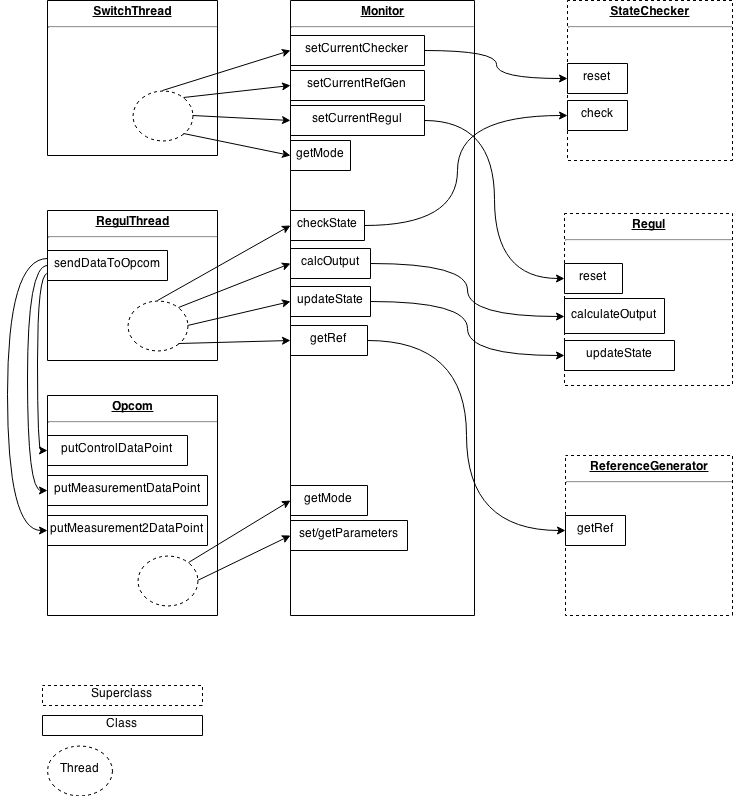
\includegraphics[width=\textwidth]{figures/UML.png}
\caption{UML of the code structure showing the classes and threads. For readability reasons superclasses are shown but not their subclasses. Some of the method names are fictive for example the method \texttt{setCurrentRegul} is referring to all the methods in the actual code that set a value to the current controller, one for each controller type}
\label{overall_fig}
\end{figure}

A few classes are not described below, as they are help classes that don't do much on their own. %kanske bara nämna vilka när vi vet vad vi faktiskt skrivit om... Tror det är PIDParameters och PlotData (och kanske OutSignal, men den kanske inte används alls)



%--------------------MISC CLASSES-----------------



\subsection{Miscellaneous classes} 	%Beskrivning av klasser som inte passar in under andra rubriker, tex Main och OpCom
%tror även Monitor bör få en snabb beskrivning här, men de flesta metoder i monitorn bör förklaras i beskrivningen av de klasser som faktiskt använder dem.
These classes don't fit under any other topic. They are found in the \texttt{main} package.

\subsubsection{Main.java}
%behöver nog inte beskrivas så ingående
This is the entry point of the program. 
All necessary objects are created, including the \texttt{Monitor}, the GUI, and all the threads.  
Once everything is set up, the threads are also started. 

\subsubsection{Monitor.java}
%behöver nog inte heller beskrivas så ingående här, bättre att skriva om den utifrån hur trådarna använder den.
This class provides sychronization between threads. Most calls to regulators and similar are done through the monitor. 
As such, the actual methods of the monitor are not very interesting in the context of this class, but rather in the context of the threads that invoke them. 
They will therefore be covered in Section \ref{Threads} where the threads are described.

The monitor also has a lot of getters and setters, for variables that need synchronization across threads.

\subsubsection{OpCom.java}
%inte så ingående heller. Vi skrev den inte, och hur den funkar beskrivs nog bättre i Operator communication.
This is a slightly modified version of \texttt{OpCom} from Lab 1. 
The actual functionality will be described in Section \ref{OpCom}. 
It communicates with the monitor, mostly through the \texttt{void set*Mode()}\footnote{The \texttt{*} is a wildcard, since there are several similar methods named by this form.} synchronized methods.



%--------------------REGULATORS-----------------




\subsection{Regulator classes}
Regulator classes determine how the control signal should be calculated, given measured states and reference values. 
They are found in the \texttt{regul} package.

\subsubsection{Regul.java}
This is the abstract superclass of all regulators. 
It has the abstract methods \texttt{calculateOutput}, \texttt{updateState} and \texttt{reset}.

\texttt{double calculateOutput(double[] measurement, double[] ref, double h)} takes the measured values, the reference values, and the period $h$ and calculates a desired control signal depending on the implementation in subclasses.

\texttt{void updateState(double h)} updates all the values that need updating before the next sample, but aren't needed to calculate the control signal for the current sample. 
This method is called after sending the control signal to the process, to minimize the delay between input and output.

The method \texttt{void reset(double[] states)} is used to reset the regulator after it has been activated, so it has relevant internal values that fit the current state of the system.

\subsubsection{BeamRegul.java}
\texttt{BeamRegul} is a PID regulator for controlling the angle of the beam. 
In addition to the implementations of the abstract methods, it also has a getter and a setter for the parameters (described by a \texttt{PIDParameters} object).

\subsubsection{BeamBallRegul.java}
This subclass is a cascaded PID regulator for controlling the position of the ball. 
It is like \texttt{BeamRegul}, except it also has a reference to a \texttt{BeamRegul} object inside itself. 
In this way, we get a simple way of describing a cascaded PID regulator. 
When calculating the control signal, this class calls the \texttt{calculateOutput} of its inner regulator. 
The same goes for updating and reseting.

%Vet inte vilka andra regulatorer som faktiskt används... Tror det bara är de där två ^



%--------------------REFERENCE GENERATORS-----------------




\subsection{Reference generator classes}
Reference generators are classes that determine where the reference values for the process should be at a particular point in time. 
Whenever a reference value is needed, it is requested from the currently chosen reference generator  (through a call to a monitor method). 
These classes are found in the \texttt{refgen} package.
 
\subsubsection{ReferenceGenerator.java}
This is the abstract superclass of the reference generators, and has the methods \texttt{double[] getRef()}, \texttt{void resetTime()} and \texttt{double getTimeSeconds()}.

\texttt{getRef()} must be implemented in subclasses, and is meant to return the current reference value.


\texttt{resetTime()} sets the starting time of the reference generator to the current time, essentially "resetting" it. 
Called whenever a reference generator is selected, but not relevant for time invariant subclasses.
%Inte säker på om denna metod används längre (av någon anledning), så isåfall bör den tas bort.
\texttt{getTimeSeconds()} gives the time in seconds since \texttt{resetTime()} was last called. 
Again not relevant for time invariant generators.

\subsubsection{ConstantRef.java}
This subclass gives a constant reference value chosen by calling \texttt{setRef(double)}. 
Which state the reference in an instance of this class refers to is given by the private variable \texttt{actualState} which is sent to the constructor at the creation of the object.

%\subsubsection{ConstantVectorRef.java}
%%Används denna?
%This class works the same as \texttt{ConstantRef}, but gives references to all states of the system.
%
%\subsubsection{ConstPosRampAngleRef.java}
%%används denna?

\subsubsection{RampRef.java}
\texttt{RampRef} gives a reference that changes linearly over time, and includes methods to set the slope and initial reference. 
Like in \texttt{ConstantRef}, a variable is used to determine which state the reference value in the current instance of the class refers to.

\subsubsection{RampToRef.java}
This subclass works almost like \texttt{RampRef}, except it stops when a chosen reference value has been reached. 
This gives a smoother reference change.

\subsubsection{RefGenGUI.java}
This is a slightly modified version of the \texttt{ReferenceGenerator} found in Lab 1, and was used for testing.

%\subsubsection{TrajectoryRef}
%%används denna?
%This subclass gives a reference that follows a curve loaded from a Matlab file.



%--------------------CHECKERS-----------------




\subsection{Checker classes}\label{Checkers}
Checker classes provide a method to determine if a state is "OK" in some way. 
We use this to find out when we should continue to the next part of the catch-throw sequence. 
These classes are found in the \texttt{checker} package.
\subsubsection{StateChecker.java}
\texttt{StateChecker} is the abstract superclass of all the checkers. It has two methods.

The method \texttt{boolean check(double[] measurement)} receives our measured values and returns a boolean describing if the state of the system fulfills some condition, depending on the implementation in subclasses.

\texttt{void reset()} is used when activating a checker to reset their internal states, so any previous usage of the object won't  affect the current workings. 
This method will be empty in subclasses that have no internal state.

%\subsubsection{BallOnBeamChecker.java}
%just nu använder vi inte den här, men det finns förändringar vi kan göra för att den ska funka

\subsubsection{ConstBallChecker.java}
This subclass checks if a ball has been around a specified point on the beam for a sufficient number of samples in a row. 
It provides the method \texttt{void setValue(double y, double tol)} for choosing the wanted stationary point and needed precision.

\subsubsection{ConstBeamChecker.java}
Almost exactly the same as \texttt{ConstBallChecker}, except for the angle of the beam. 
It does, however, not have the ability to change the tolerance. 

\subsubsection{LEDChecker.java}
Checks if the beam is in the pickup position - in other words if the LED is on. 
This is done by actually reading the digital in channel.

\subsubsection{Null checker}
Though not a class, the monitor has the ability to set the "null checker", which is roughly equivalent to turning off checking. 
This is not needed, since calling a checker when SwitchThread is not waiting or ready to run does nothing except waste time, but it can avoid unneccesary processor load to some extent.




%--------------------THREADS-----------------




\subsection{Threads}\label{Threads}

\subsubsection{RegulThread.java}
This is the main regulator loop. Every loop iteration, this thread does the following things (in order):
\begin{itemize}
\item reads input from process
\item calculates output
\item sends output to process
\item sends data to the GUI
\item updates the state of the regulator
\item checks the state of the system
\end{itemize}

Except for reading and sending, these things are done by calling methods in \texttt{Monitor}. 
As such, their exact functionalities depend on which settings have been chosen in the monitor. 
This thread runs oblivious of changes to the settings, and has no need to know of them; the basic structure of the loop remains the same.

When the thread calls the synchronized method \texttt{double calcOutput(double[] measurement)}, the result is calculated using \texttt{currentRegul} in the monitor. 
Depending on monitor calls from other threads (namely \texttt{SwitchThread} and \texttt{OpCom}), the actual object \texttt{currentRegul} points to will be different. 
In the same way, the reference values needed to do the output calculations are received from \texttt{currentRefGen}, which also points to different objects depending on the wanted functionality.

"Checking" the state of the system means to evaluate if the system fulfils certain criteria. 
The actual criteria, again, depend on settings given to the monitor. 
If the state is deemed "ok", waiting threads (in our case, \texttt{SwitchThread}) are awoken. 
Otherwise, nothing happens. More details in Sections \ref{SwitchThread} and \ref{Checkers}.



\subsubsection{SwitchThread.java}\label{SwitchThread}
\texttt{SwitchThread} is the thread that handles our sequence mode.

It uses monitor calls to change regulators and reference generators to modify the behaviour of the process. 
It also uses checker classes to wait for certain events to happen, or \texttt{Thread.sleep()} in case a certain amount of time needs to pass.

Changing of regulators is done through the \texttt{set*Regul()} monitor methods, while reference generators are set through the \texttt{setRefGen*()} methods. 
In the reference generator case, the arguments are different depending on the reference generator. 
Changing of regulators and reference generators is generally done within a single synchronized block.

When the thread calls the synchronized methods \texttt{void set*Check}, where \texttt{*} and arguments depend on the particular checker wanted, the monitor's \texttt{stateChecker} is set to an instance of the wanted checker, the relevant settings in the chosen checker are set, and the thread calls \texttt{wait()}. 
The responsibility of waking this thread up now falls to \texttt{RegulThread}, which polls the currently selected checker every iteration. 
If the polled checker returns \texttt{true}, it wakes all waiting threads up, allowing \texttt{SwitchThread} to continue executing. 
In this way, this thread knows the state of the system is satisfactory to continue with the sequence once it wakes up.

The thread can also wake up if sequence mode is turned off, in which case the thread will go back to the starting position and wait to be turned on again.

This thread also handles the digital output, shooting out a ball when the process is ready to receive it.

The general structure of a segment is
\begin{itemize}
\item set a regulator,
\item set a reference generator,
\item set a checker and wait to wake up
\end{itemize}

Of course, the different parts need to go together: if you set the regulator to regulating the beam, 
the reference generator should also give a reference for the beam, 
and the checker needs to wait for a state that will actually be achieved.

After the ball has been weighed, the checkers are no longer used, and instead beam angle changes in combination with sleeps handle the throwing.
